\section{Spektroskopie der Hyperfeinstruktur von Rubidium}
\subsection{Durchführung}
Bei der Messung des Hyperfein-Absorptionsspektrums befinden sich die beiden Linsen und
die Rubidiumzelle im Strahlengang.
Der Konstantanteil des Laserstroms, Modulationsamplitude und -frequenz
sind wie bei der Messung der Zeitabhängigkeit der Laserfrequenz (\autoref{sect:durchführung}).
Äußere Magnetfelder bleiben unkompensiert, weil die Zeeman-Aufspaltung der Hyperfeinstruktur im Erdmagnetfeld
mit der Linienbreite der Laserdiode nicht auflösbar ist.
Die Messung wird auf der steigenden und der fallenden Flanke der Modulationsspannung durchgeführt.


\subsection{Auswertung}
Da in dieses Teil der Auswertung häufiger Kurvenanpassungen mit einer Gauß-Funktion durchgeführt werden, wird folgende Konvention eingeführt:
\begin{equation}
    \label{eq:convention:gauss}
    \gaus(x; A, \mu, \sigma) = A \cdot e^{-\frac{1}{2} \left( \frac{x-\mu}{\sigma} \right)^2}
\end{equation}
\subsubsection*{Frequenzkalibrierung}
Das Etalonspektrum und die Spannung der Lasermodulation sind in \autoref{img:etalon:fit} abgebildet. 
Die Peaks des Etalonspektrums werden mit Gauß-Kurven und einem linearen Untergrund gefittet. 
\begin{equation}
    U_\text{ph}(t) = a + b \cdot t + \gaus(t; A, \mu, \sigma)
\end{equation}
Des Weiteren wird die Spannung für die Lasermodulation mit einer Geraden gefittet.
\begin{equation}
    U_\text{L} = a + \cdot t
\end{equation}
\begin{figure}[H]
\begin{center}
  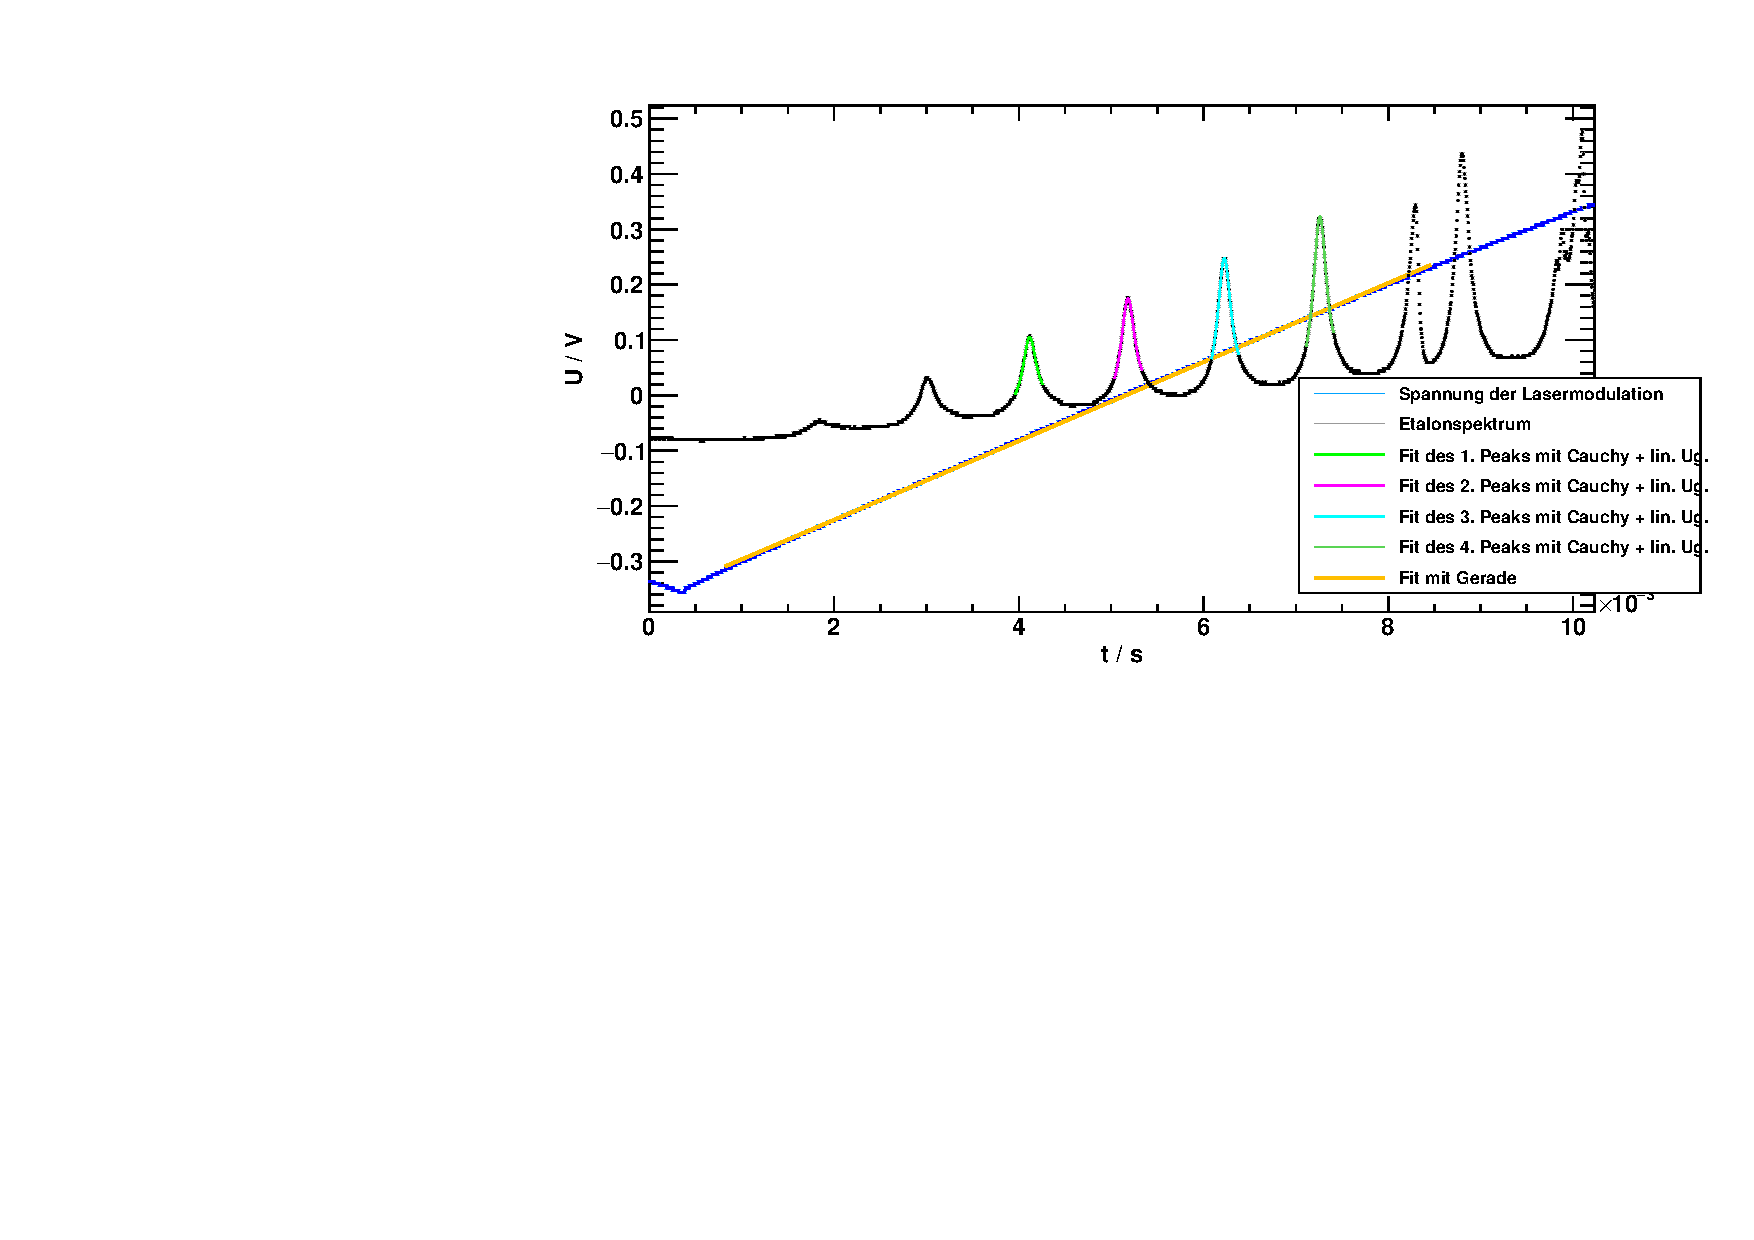
\includegraphics[width=\textwidth]{../img/part2/up-etalon_zoom_fit.pdf}
  \caption{caption.}
  \label{img:etalon:fit}
\end{center}
\end{figure}
TODO: Farbcode ändern \\
Gerade von $U_\text{L}$ wird nur betrachtet, um zu kontrollieren, ob die Spannung auch gerade ansteigt. \\
TODO: Tabelle mit Peakdaten \\
TODO: Mehr peaks fitten, wenn möglich

Aus dem freien Spektralbereich des Etalons $\Delta \nu_\text{FSR} = 9924 \pm 30\,\text{MHz}$ lässt sich nun die Differenz der Laserfrequenz bei den verschiedenen 
Peaks bestimmen. Der erste Peak wird als Referenzpeak festgelegt. Der Frequenzabstand $\nu_i$ zwischen erstem und $i$-ten Peak lässt sich nun 
folgendermaßen berechnen\footnote{Gedankenspiel zur Fehlerrechnung: Interpretiert man $2 \cdot a$ als $a + a$, so ist der Fehler im ersten Fall $2 \cdot s_a$, im zweiten 
allerdings $\sqrt{2} \cdot s_a$, wenn man die Autokorrelation von $a$ nicht berücksichtigt. Mit $\cor(a, a) = 1$ 
erhält man $\sqrt{s_a^2 + s_a^2 + 2 \cdot s_a \cdot s_a \cdot \cor(a, a)} = 2 \cdot s_a$.}: 
\begin{equation}
    \Delta \nu_i = \Delta \nu_\text{FSR} \cdot i, \qquad s_{\Delta \nu_i} = \sqrt{i} \cdot s_{\Delta \nu_\text{FSR}} 
\end{equation}
Die Frequenzabstände werden nun gegen die Maximumspositionen (also die Erwartungswerte der Gauß-Funktionen) der Etalonpeaks aufgetragen ( \autoref{img:etalon:calibration}).
\begin{figure}[H]
\begin{center}
  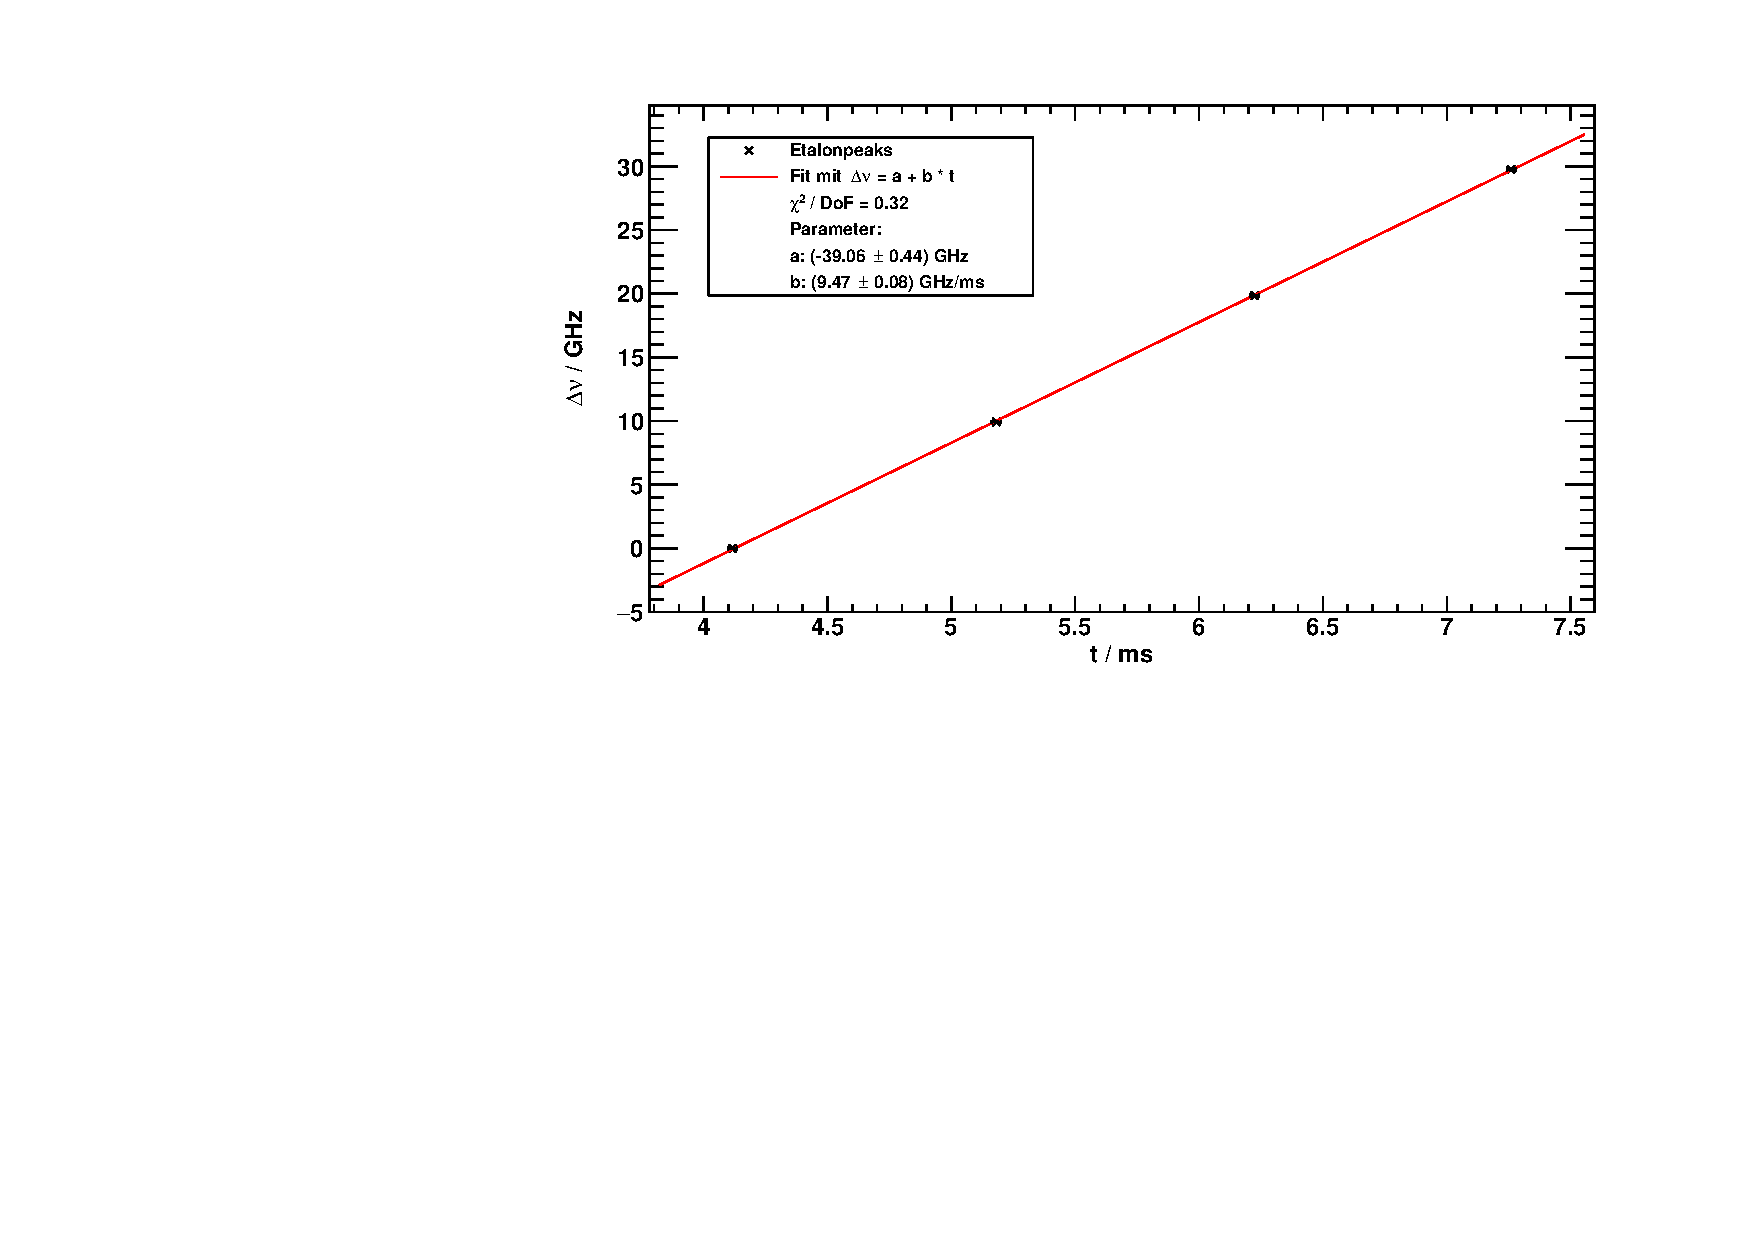
\includegraphics[width=\textwidth]{../img/part2/up-etalon_zoom-etalon_calibration.pdf}
  \caption{caption.}
  \label{img:etalon:calibration}
\end{center}
\end{figure}
Aus dem Fit mit einer Geraden 
\begin{equation}
    \Delta \nu(t) = a + r \cdot t  %TODO Parameter in Plot ändern
\end{equation}
lässt sich nun die Scanrate $r$ bestimmen. Man erhält %TODO Bessere Variable für Scanrate
\begin{equation}
    r = (9.40 \pm 0.02)\,\frac{\text{GHz}}{ms}\ \, .
\end{equation}

\subsubsection*{Hyperfeinstruktur-Übergänge}
nur 6 peaks erkennbar, da 2 nicht aufgelößt werden können \\
fit mit überlagerten Gauß \\
tabelle mit peak-positionen
\begin{figure}[H]
\begin{center}
  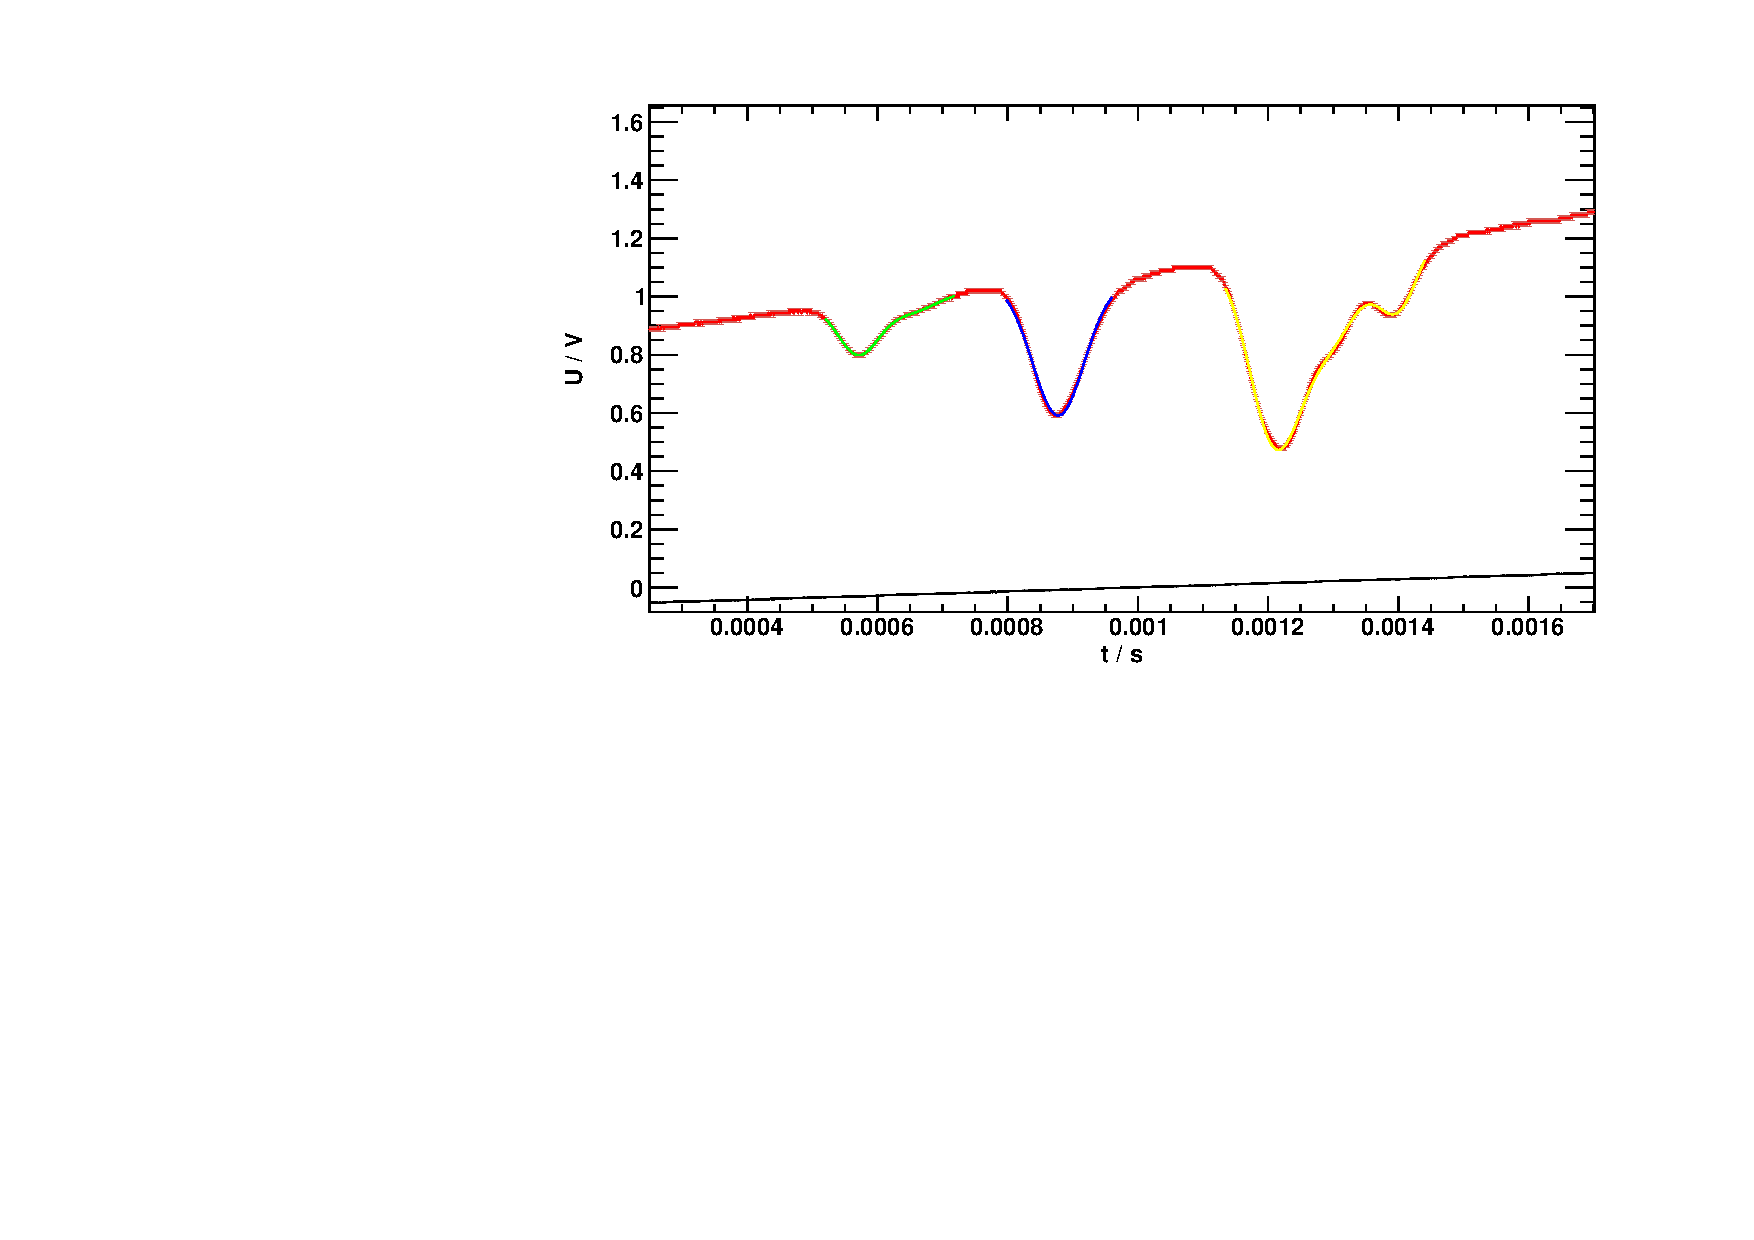
\includegraphics[width=\textwidth]{../img/part2/up-hfs_zoom_fit.pdf}  %TODO Better start params
  \caption{caption.}
  \label{img:hfs:fit:up}
\end{center}
\end{figure}

\subsubsection*{Berechnung des Spektrums}
festlegung referenzpeak \\
berechnung des spektrums 

\subsubsection*{Vergleich mit den Literaturwerten}
Tabelle mit Spektrumswerten (Literaturwert, aufsteigend, absteigend (eine Tabelle))
Gerade sollte Steigung 1 und Achsenabschnitt 0 Ghz haben

\begin{figure}[H]
\begin{center}
  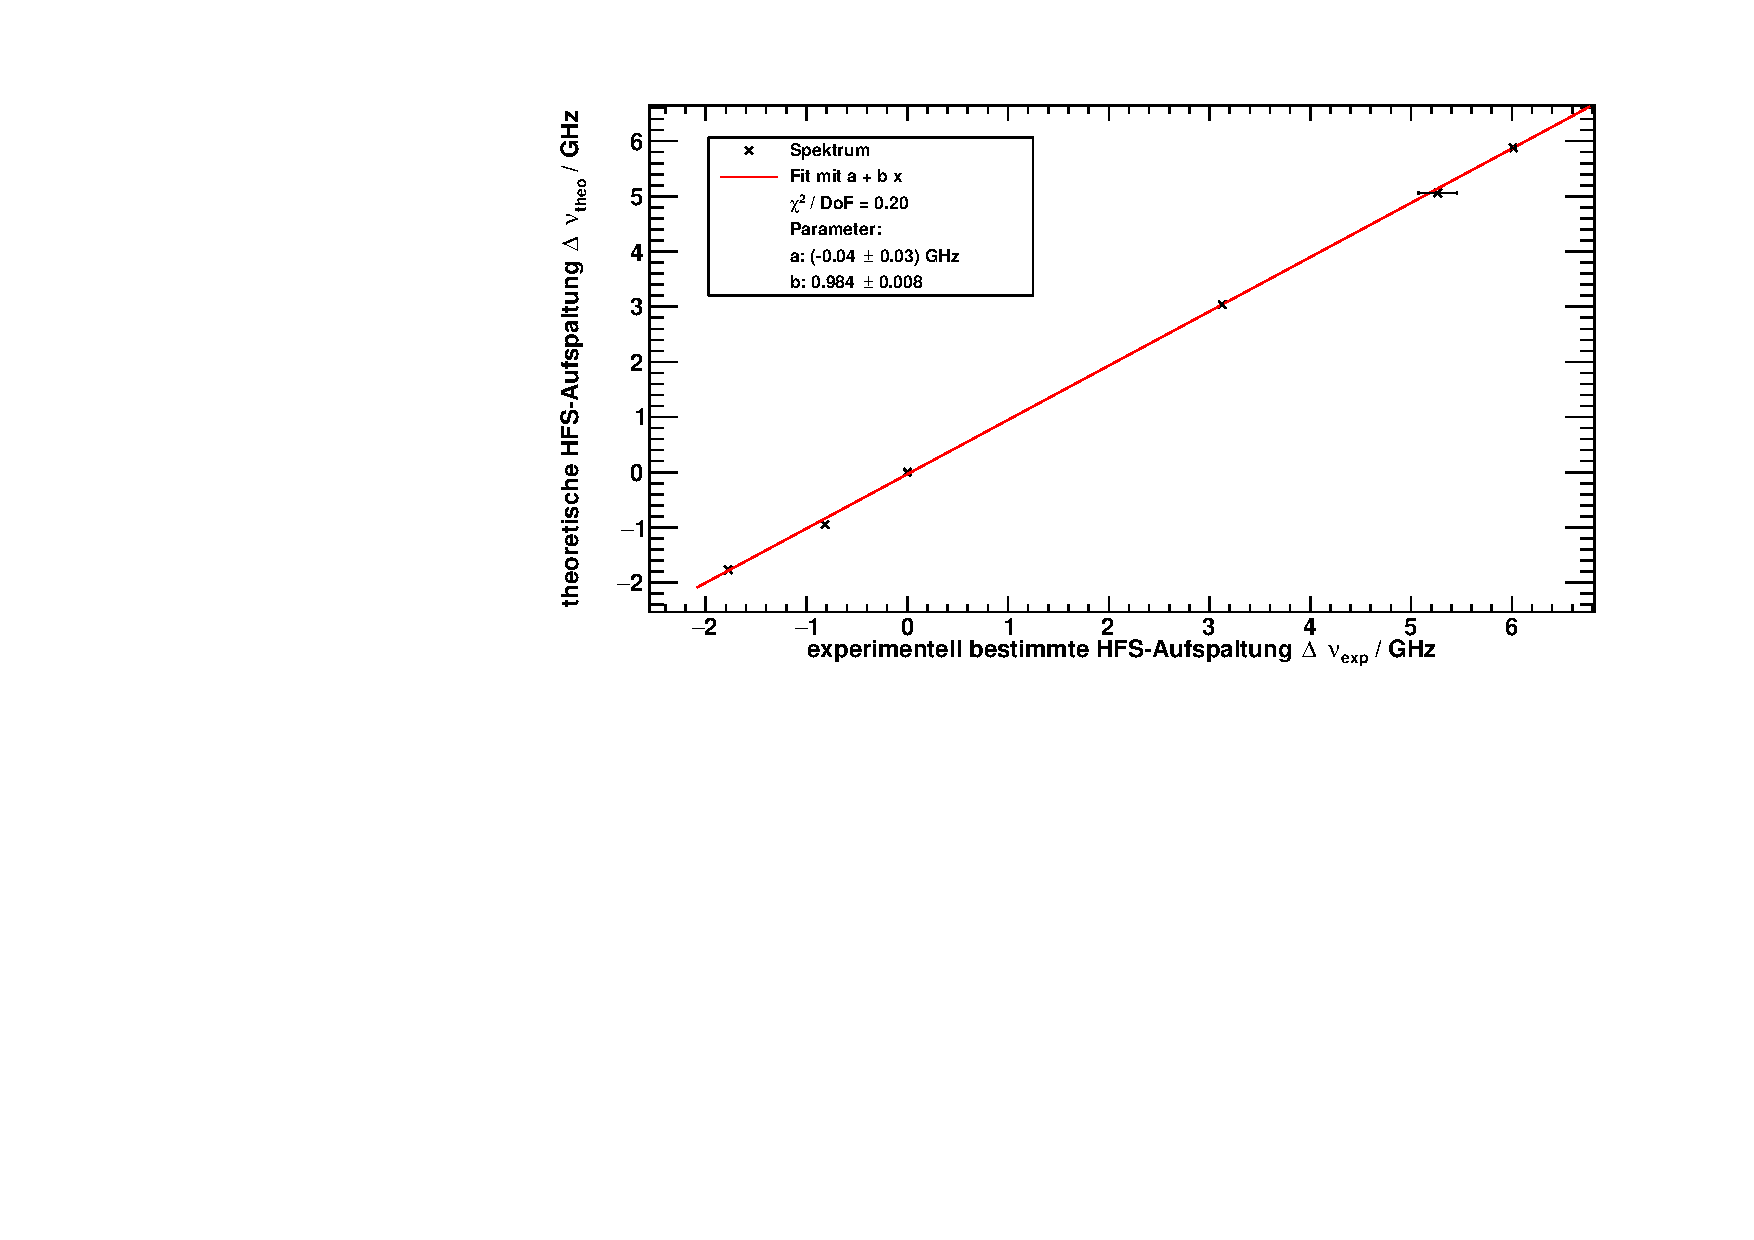
\includegraphics[width=\textwidth]{../img/part2/up-spectrum.pdf}
  \caption{caption.}
  \label{img:hfs:spectrum:up}
\end{center}
\end{figure}

\begin{figure}[H]
\begin{center}
  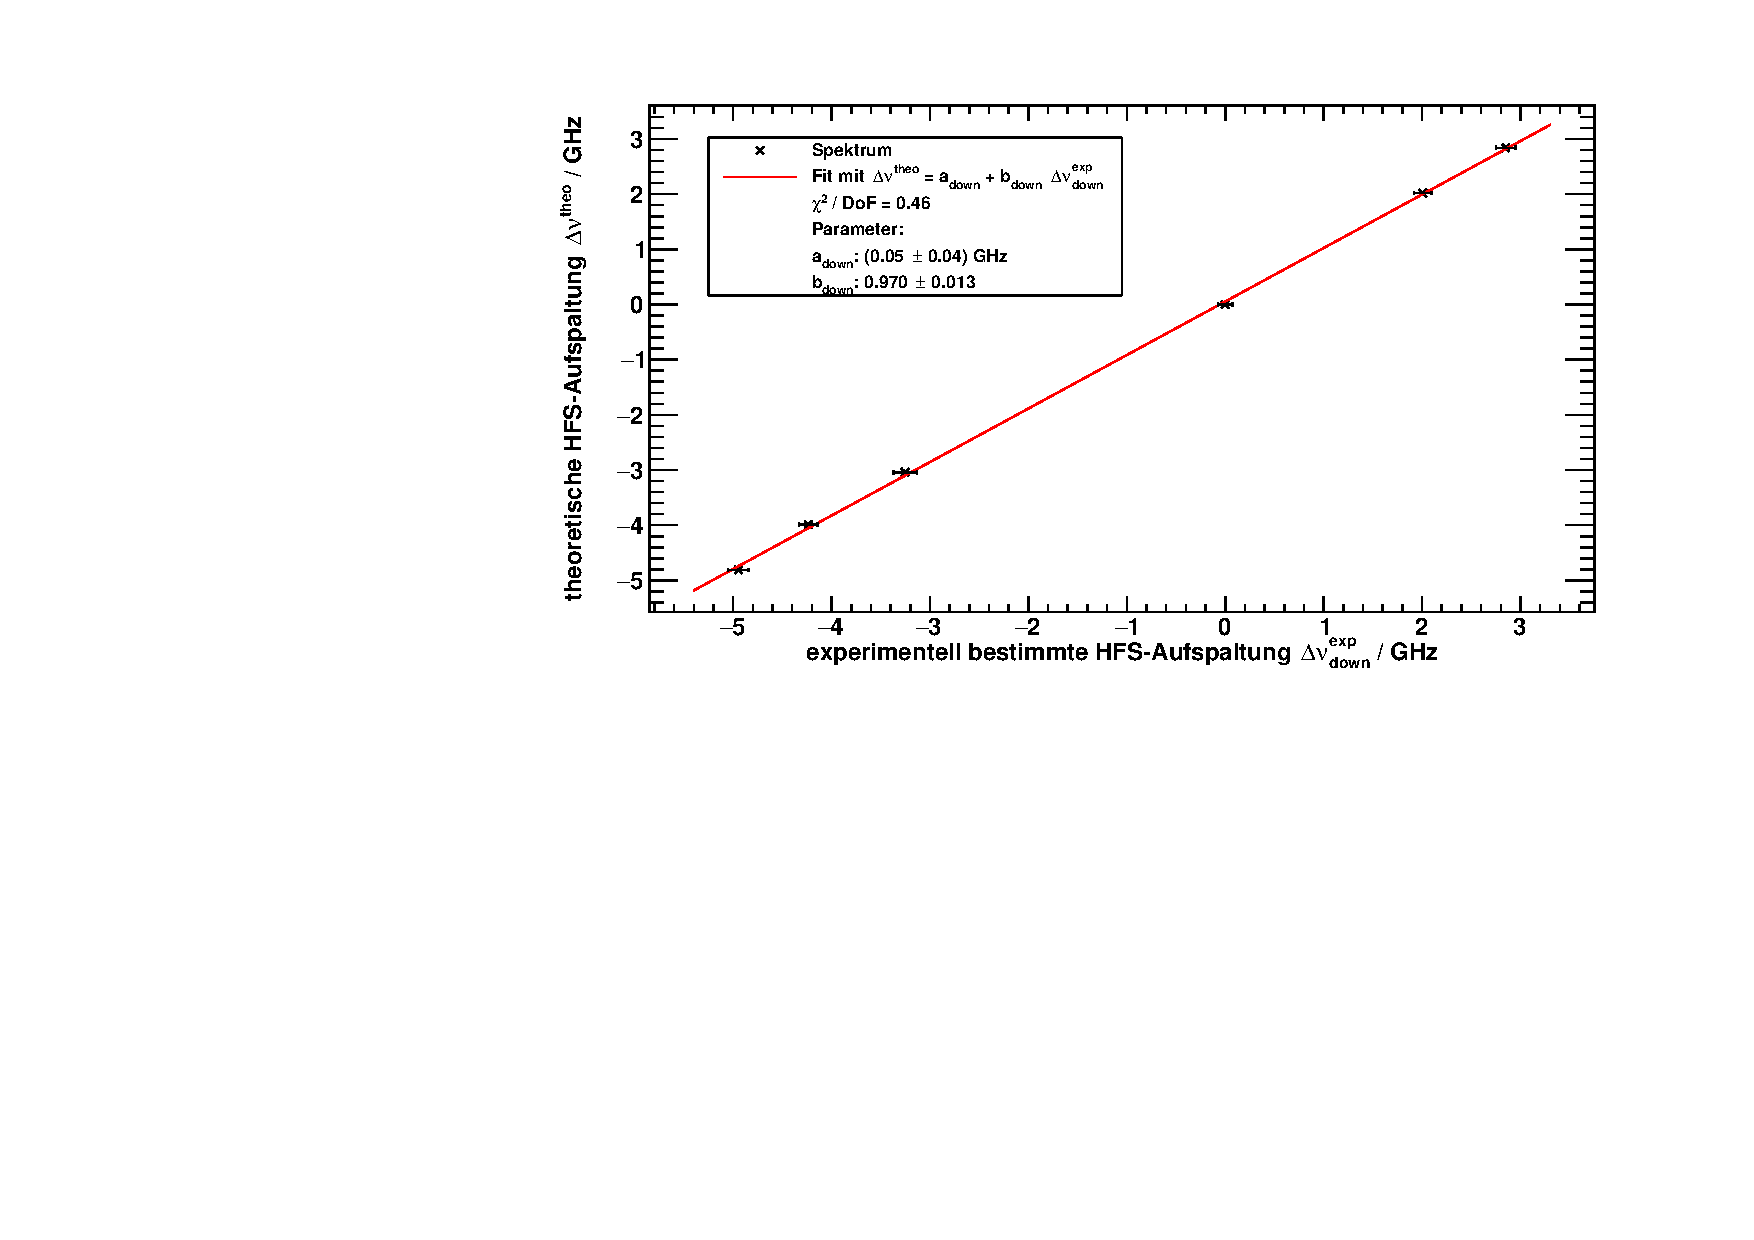
\includegraphics[width=\textwidth]{../img/part2/down-spectrum.pdf}
  \caption{caption.}
  \label{img:hfs:spectrum:down}
\end{center}
\end{figure}
